% --------------------------------------------------------------
% This is all preamble stuff that you don't have to worry about.
% Head down to where it says "Start here"
% --------------------------------------------------------------
 
\documentclass[12pt]{article}
 \usepackage{graphicx}
\usepackage[margin=1in]{geometry} 
\usepackage{amsmath,amsthm,amssymb}
\usepackage{algorithmic, mathtools}
\newcommand{\N}{\mathbb{N}}
\newcommand{\Z}{\mathbb{Z}}
 
 
\begin{document}
 
% --------------------------------------------------------------
%                         Start here
% --------------------------------------------------------------
 
%\renewcommand{\qedsymbol}{\filledbox}
 
\title{Homework \#11}%replace X with the appropriate number
\author{\\ %replace with your name
CPSC 395 - Analysis of Algorithms
\\ Due: Monday, 3} %if necessary, replace with your course title
\date{}
\maketitle

For your diagrams, you can do it by hand, then insert the pictures into your pdf.

\begin{enumerate}
\item Exercise 24.1-1 \\
Run the Bellman-Ford algorithm on the directed graph of Figure 24.4, using vertex z as the source. In each pass, relax edges in the same order as in the figure, and show the d and $\pi$ values after each pass. Now, change the weight of edge (z,x) to 4 and run the algorithm again, using s as the source. The order of relaxation is (t,x),(t,y),(t,z),(x,t),(y,x),(y,z),(z,x),(z,s),(s,t)(s,y). There are $\abs{V}-1$ iterations, so since there are 5 vertices there are 4 iterations.\\

Vertex Z as the source: \\
First iteration- The edges relaxed are (z,x),(z,s),(s,t),(s,y). S.d = 2, X.d = 7, T.d = 8, Y.d = 9. That's the end of the first iteration.\\
Second iteration- The edges relaxed are (x,t),(y,x),. T.d = 5, X.d = 6. That's the end of the second iteration.\\
Third iteration- The edges relaxed are (x,t). T.d = 4. That's the end of the third iteration.\\
Fourth iteration- No edge is relaxed and this is the last iteration.\\
\begin{center}
 \begin{tabular}{|c|c c c c c|} 
 \hline
 Pass & s(d,$\pi$) & t(d,$\pi$) & x(d,$\pi$) & y(d,$\pi$) & z(d,$\pi$)\\ [0.5ex] 
 \hline
 0 &$\infty$,NIL &  $\infty$,NIL & $\infty$.NIL & $\infty$,NIL & 0,NIL\\ 
 \hline
 1 & 2,z & 8,s & 7,z & 9,s & 0,NIL \\
 \hline
 2 & 2,z & 5,x & 6,y & 9,s & 0,NIL \\
 \hline
 3 & 2,z & 4,x & 6,y & 9,s & 0,NIL \\
 \hline
 4 & 2,z & 4,x & 6,y & 9,s & 0,NIL \\
 \hline
\end{tabular}
\end{center}
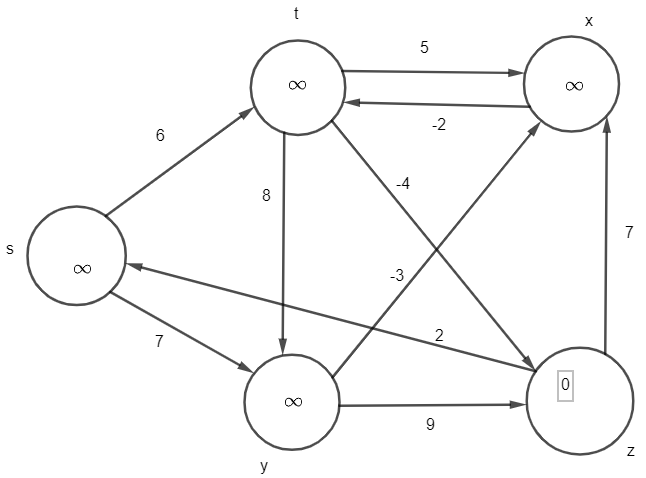
\includegraphics[scale=.65]{24.1-1 Vertex Z/1-1Z.png}\\
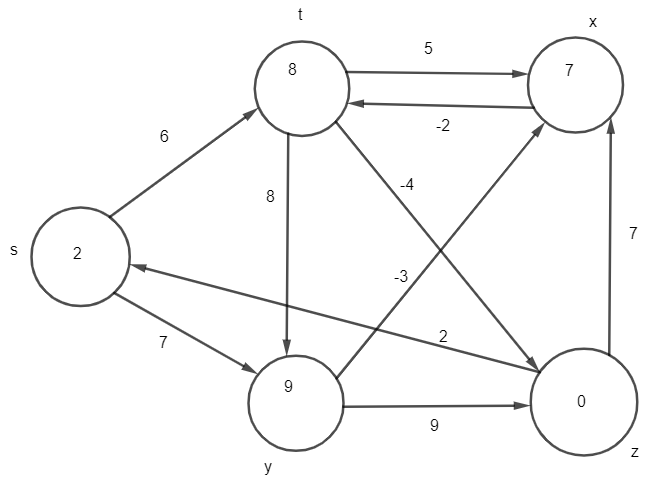
\includegraphics[scale=.65]{24.1-1 Vertex Z/First Iteration.png}\\
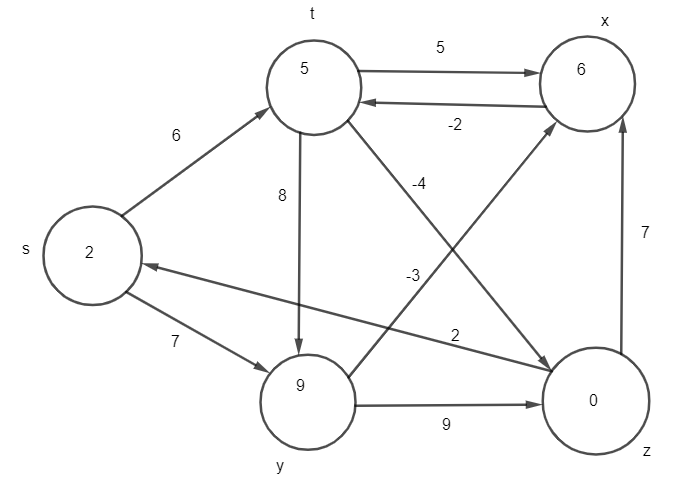
\includegraphics[scale=.65]{24.1-1 Vertex Z/Second Iteration.png}\\
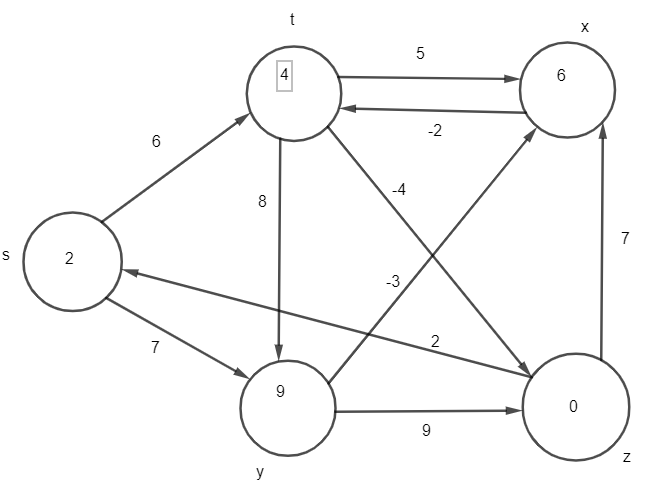
\includegraphics[scale=.65]{24.1-1 Vertex Z/Third Iteration.png}\\
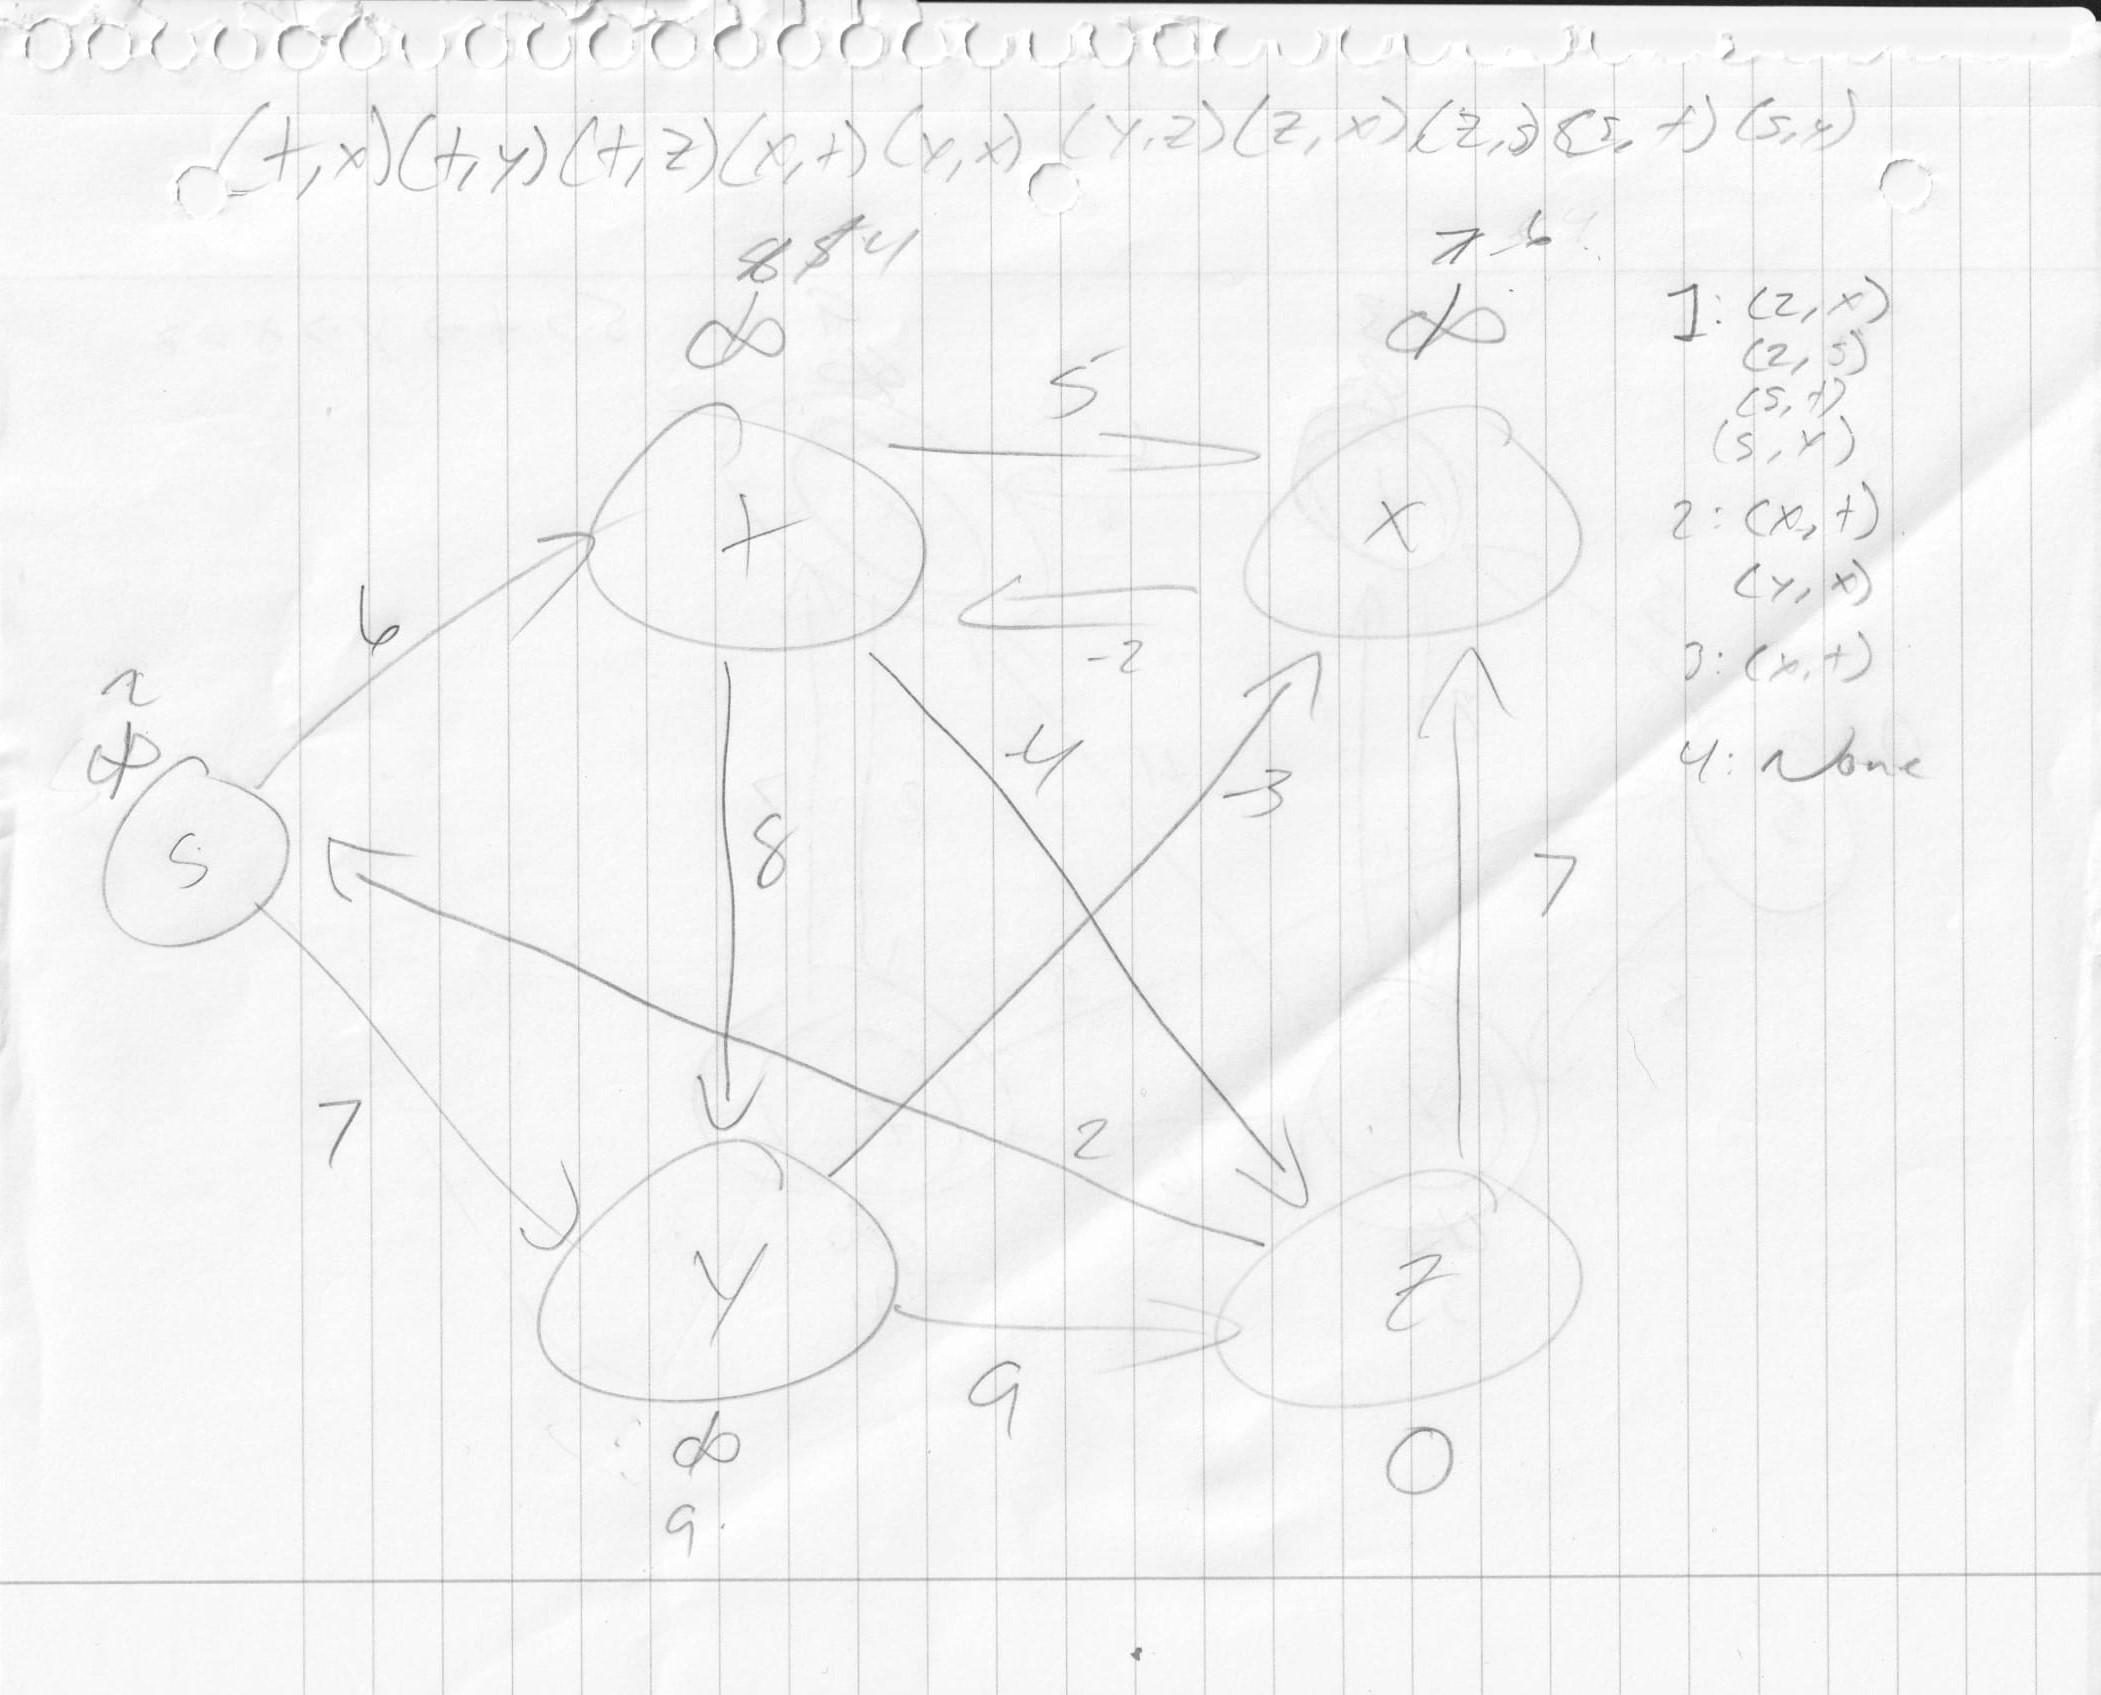
\includegraphics[scale=.32]{24.1-1 Vertex Z/24.1-1Z.jpg}

Weight of edge (z,x) is 4 and s is the source: \\
First iteration - Edges (s,t) and (s,y) are relaxed. T.d = 6 and Y.d = 7. End of first iteration.\\
Second iteration - Edges relaxed are (t,x),(t,z)(y,x). X.d = 11 and with (y,x) becomes 4, Z.d = 2. End of second iteration\\
Third iteration- Edges relaxed are (x,t). T.d = 2. End of third iteration.\\
Fourth iteration- Edges relaxed are (t,z),(z,x). Z.d = -2, X.d = 2. End of fourth iteration. There's a negative weight cycle so it will return false.\\
\begin{center}
 \begin{tabular}{|c|c c c c c|} 
 \hline
 Pass & s(d,$\pi$) & t(d,$\pi$) & x(d,$\pi$) & y(d,$\pi$) & z(d,$\pi$)\\ [0.5ex] 
 \hline
 0 & 0,NIL &  $\infty$,NIL & $\infty$,NIL & $\infty$,NIL & $\infty$,NIL\\ 
 \hline
 1 & 0,NIL & 6,s & $\infty$,NIL & 7,s & $\infty$,NIL \\
 \hline
 2 & 0,NIL & 6,s & 4,y & 7,s & 2,t \\
 \hline
 3 & 0,NIL & 2,x & 4,y & 7,s & 2,t \\
 \hline
 4 & 0,NIL & 2,x & 2,z & 7,s & -2,t \\
 \hline
\end{tabular}
\end{center}
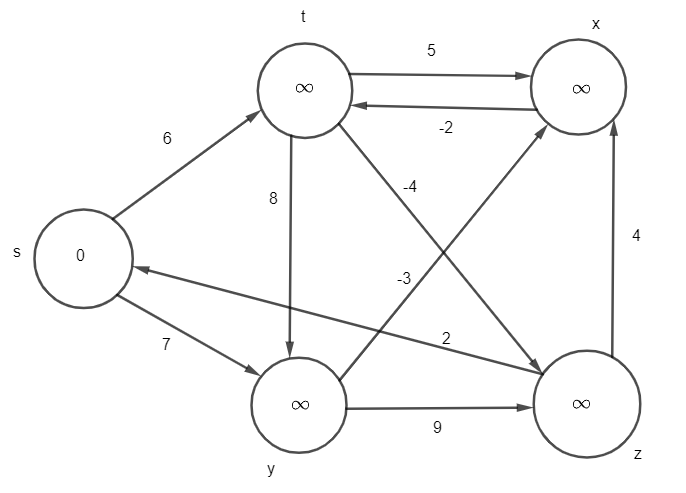
\includegraphics[scale=.65]{24.1-1 Vertex S/1-2.png}\\
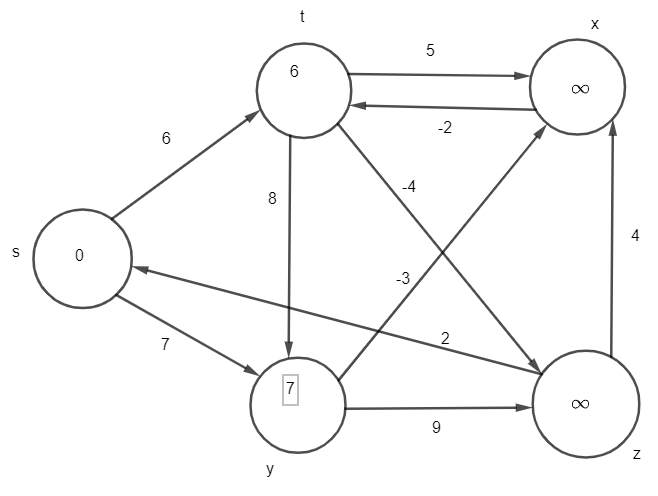
\includegraphics[scale=.65]{24.1-1 Vertex S/1-2 First iteration.png}\\
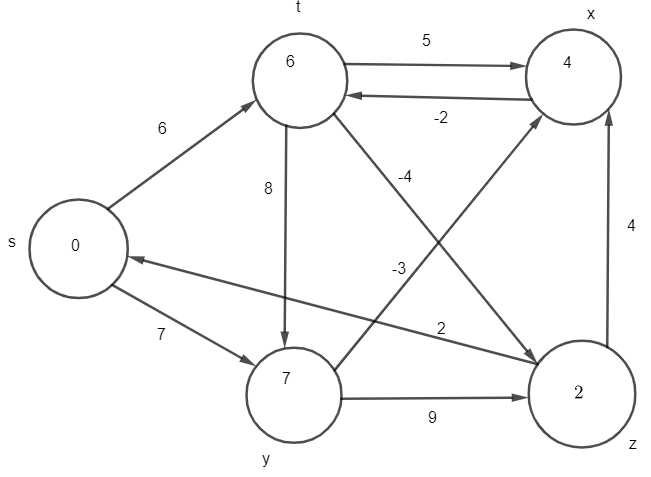
\includegraphics[scale=.65]{24.1-1 Vertex S/1-2 Second iteration.png}\\
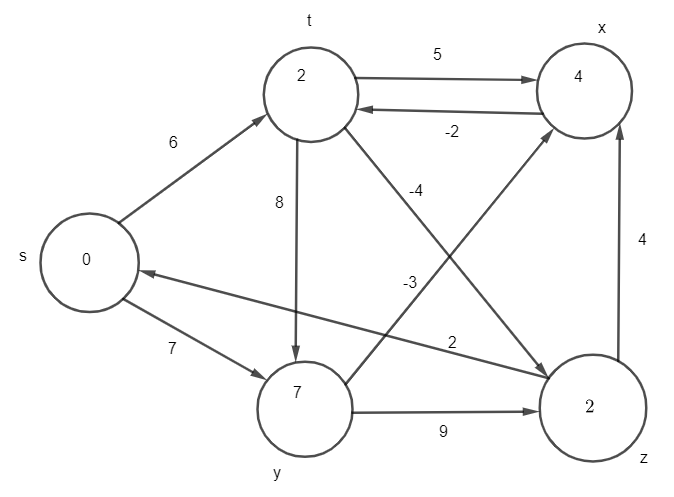
\includegraphics[scale=.65]{24.1-1 Vertex S/1-2 third iteration.png}\\
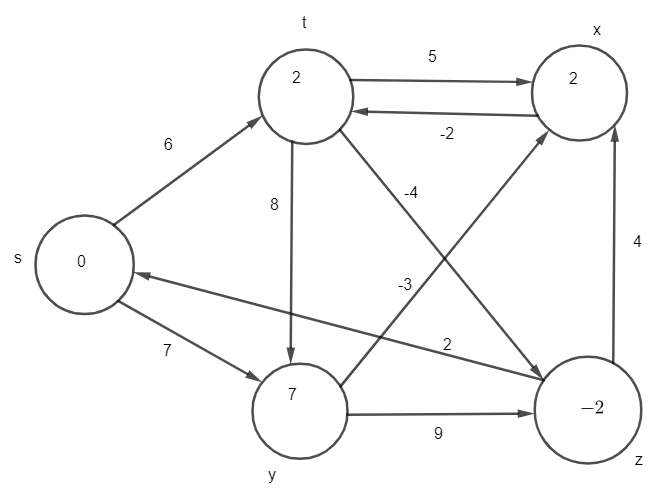
\includegraphics[scale=.65]{24.1-1 Vertex S/1-2fourth iteration.png}\\
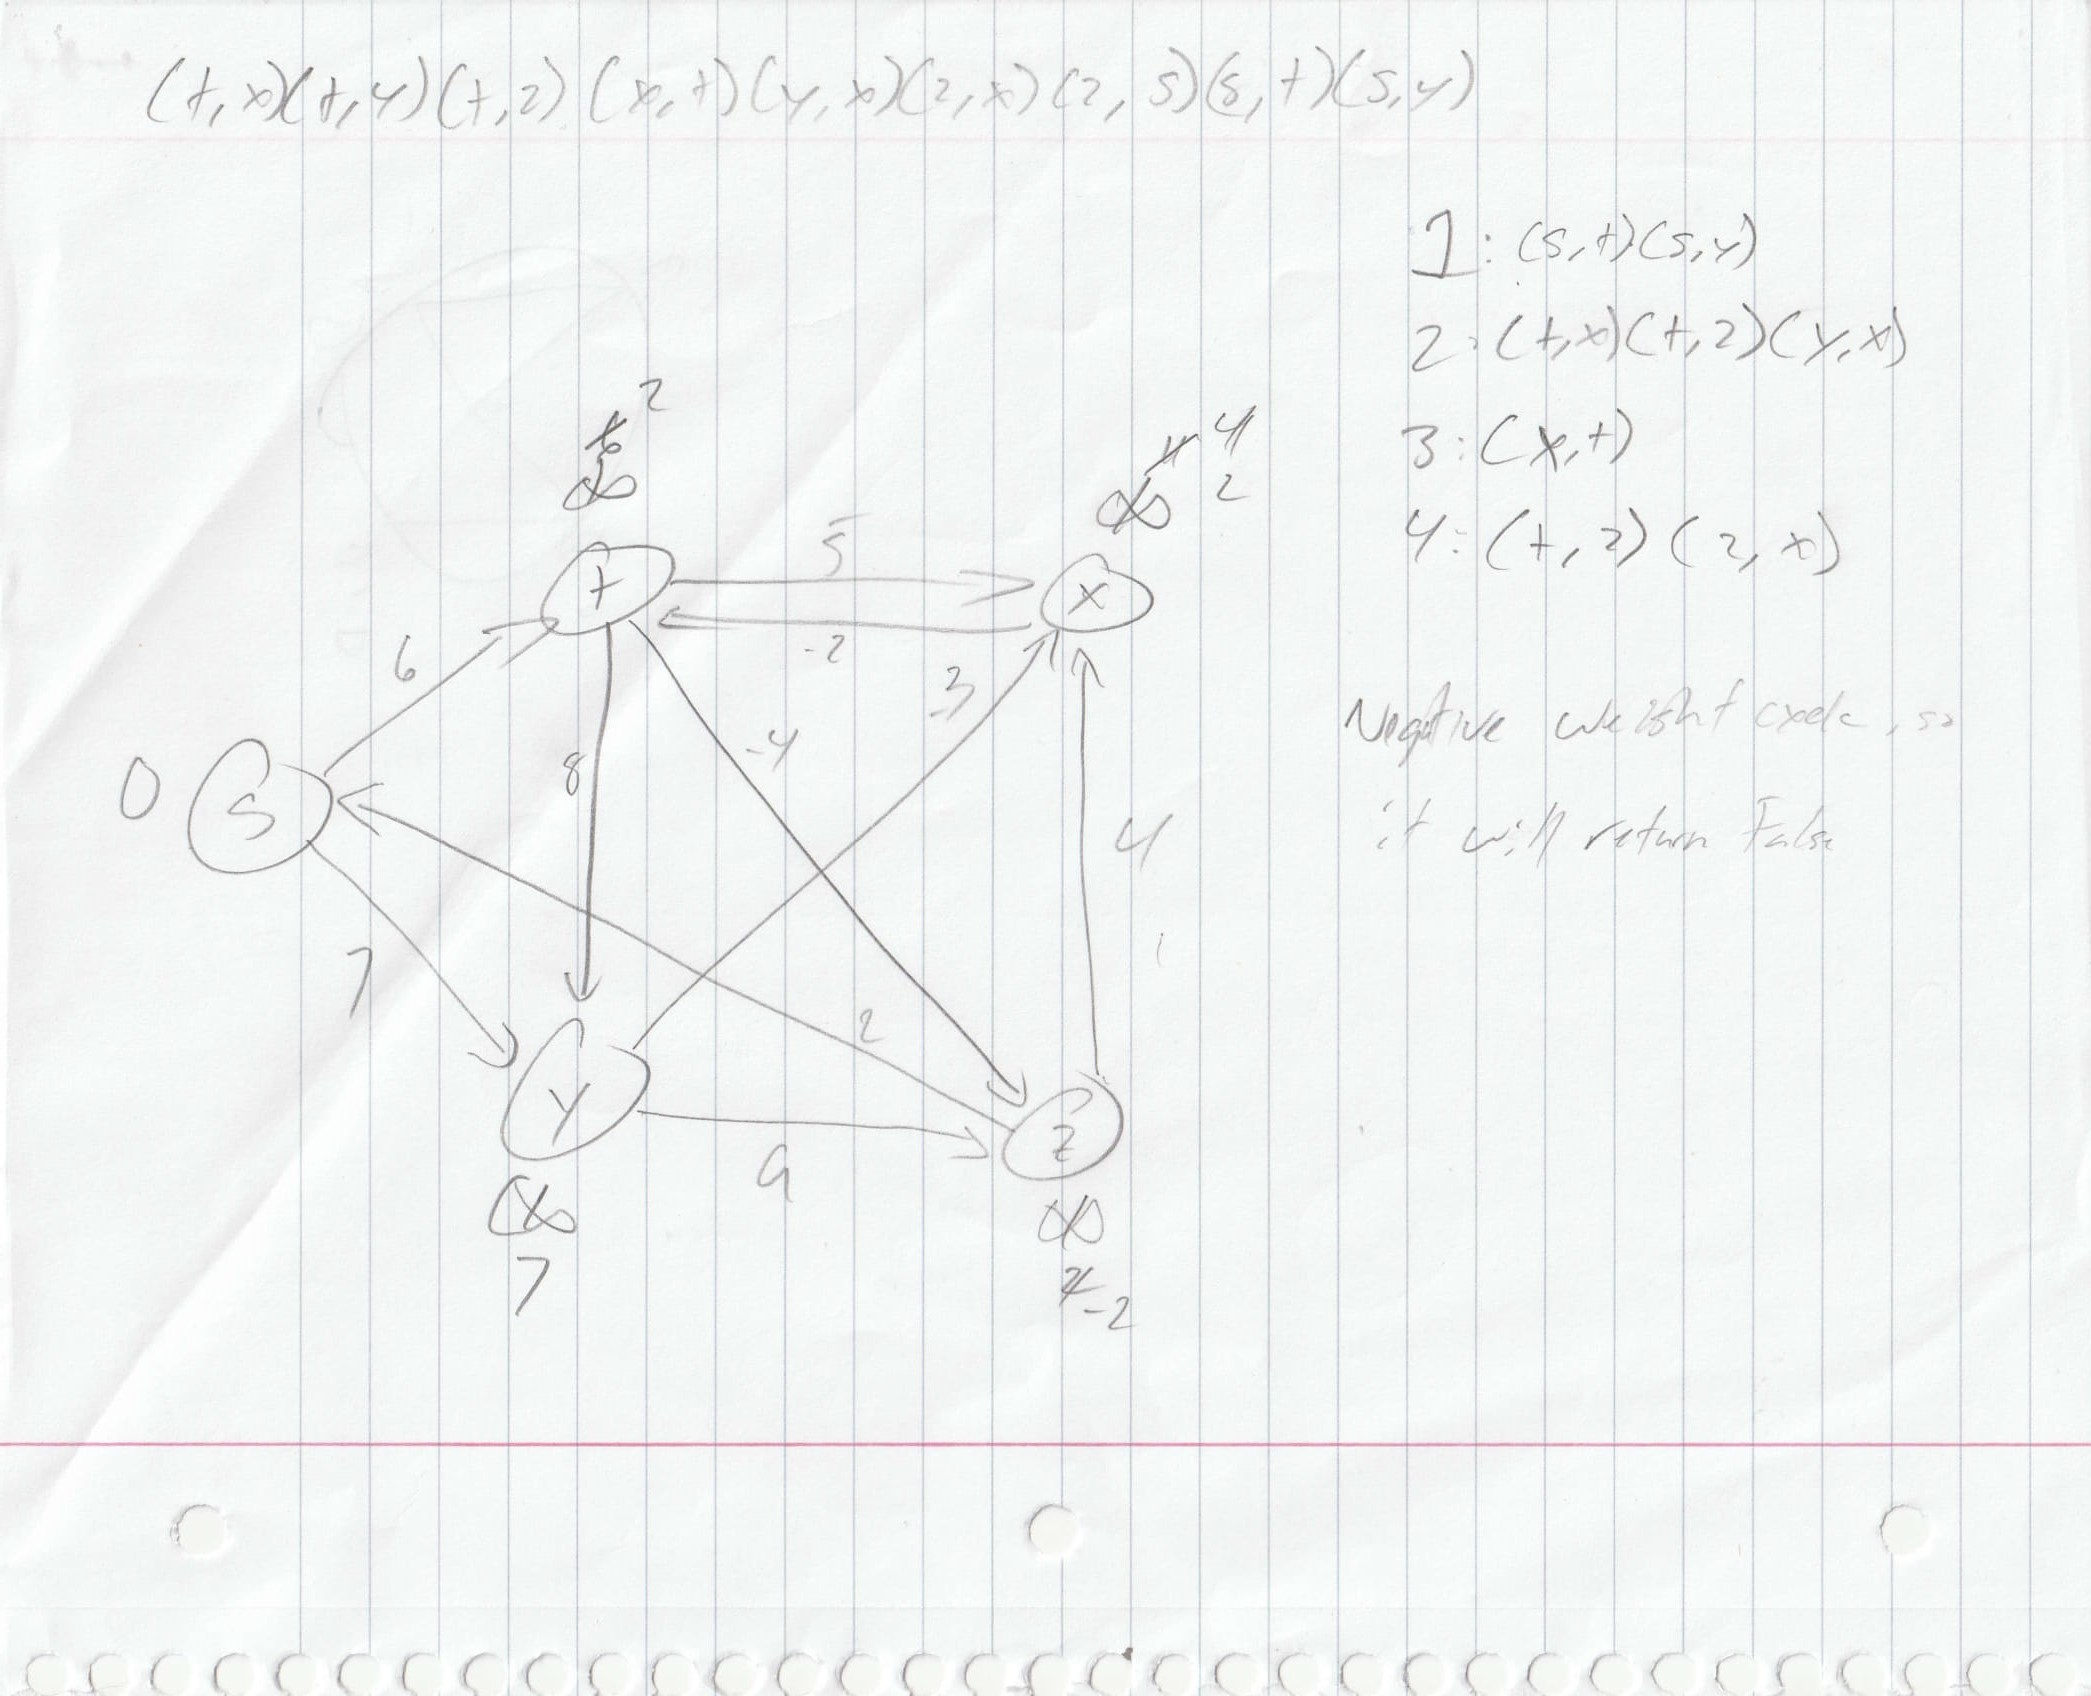
\includegraphics[scale=.32]{24.1-1 Vertex S/24.1-1S.jpg}

\item Exercise 24.1-4 \\
Modify the Bellman-Ford algorithm so that it sets v.d to $-\infty$ for all vertices v for which there is a negative-weight cycle on some path from the source to v. \\
Original Bellman-Ford algorithm: \\
BELLMAN-FORD(G,w,s)
\begin{algorithmic}
    \STATE INITIALIZE-SINGLE-SOURCE(G,s)
    \FOR{i = 1 to $\abs{\lvert}G.V{\rvert}$ -1}
        \FOR{each edge (u,v) $\in$ G.E}
            \STATE RELAX(u,v,w)
        \ENDFOR
    \ENDFOR
    \FOR{each edge (u,v) $\in$G.E}
        \IF{v.d $>$ u.d + w(u,v)}
            \STATE return FALSE
        \ENDIF
    \ENDFOR
    \STATE return TRUE
\end{algorithmic}

The second for loop is for finding the negative-weight cycles and upon finding them returns false. So it simply must be changed to set v.d to $-\infty$

MODIFIED-BELLMAN-FORD(G,w,s)
\begin{algorithmic}
    \STATE INITIALIZE-SINGLE-SOURCE(G,s)
    \FOR{i = 1 to $\abs{\lvert}G.V{\rvert}$ -1}
        \FOR{each edge (u,v) $\in$ G.E}
            \STATE RELAX(u,v,w)
        \ENDFOR
    \ENDFOR
    \FOR{each edge (u,v) $\in$G.E}
        \IF{v.d $>$ u.d + w(u,v)}
            \STATE v.d = $-\infty$
        \ENDIF
    \ENDFOR
    \STATE return TRUE
\end{algorithmic}


\item Exercise 24.2-1 \\
Run DAG-SHORTEST-PATHS on the directed graph of Figure 24.5, using vertex r as the source. \\
Vertex r is the source. S.d = 5 and t.d = 3.\\
Vertex s is selected after r. X.d = 11 and t.d stays 5 since 5 < 7. \\
Vertex t is selected after s. Y.d = 7 (t.d + 4), z.d = 5 (t.d + 2), x.d = 10 (10 < 11).\\
Vertex x is selected after t. Nothing is changed. \\
Vertex y is selected after x. Nothing is changed. \\
Vertex z is selected after y. Nothing is changed.\\
\begin{center}
 \begin{tabular}{|c|c c c c c|} 
 \hline
 Selected Vertex & s(d) & t(d) & x(d) & y(d) & z(d)\\ [0.5ex] 
 \hline
 NIL & 0 &$\infty$ &  $\infty$ & $\infty$ & $\infty$\\ 
 \hline
 r & 5 & 3 & $\infty$ & $\infty$ & $\infty$\\
 \hline
 s & 5 & 3 & 11 & $\infty$ & $\infty$ \\
 \hline
 t & 5 & 3 & 10 & 7 & 5\\
 \hline
 x & 5 & 3 & 10 & 7 & 5\\
 \hline
 y & 5 & 3 & 10 & 7 & 5\\
 \hline
 z & 5 & 3 & 10 & 7 & 5 \\
 \hline
\end{tabular}
\end{center}
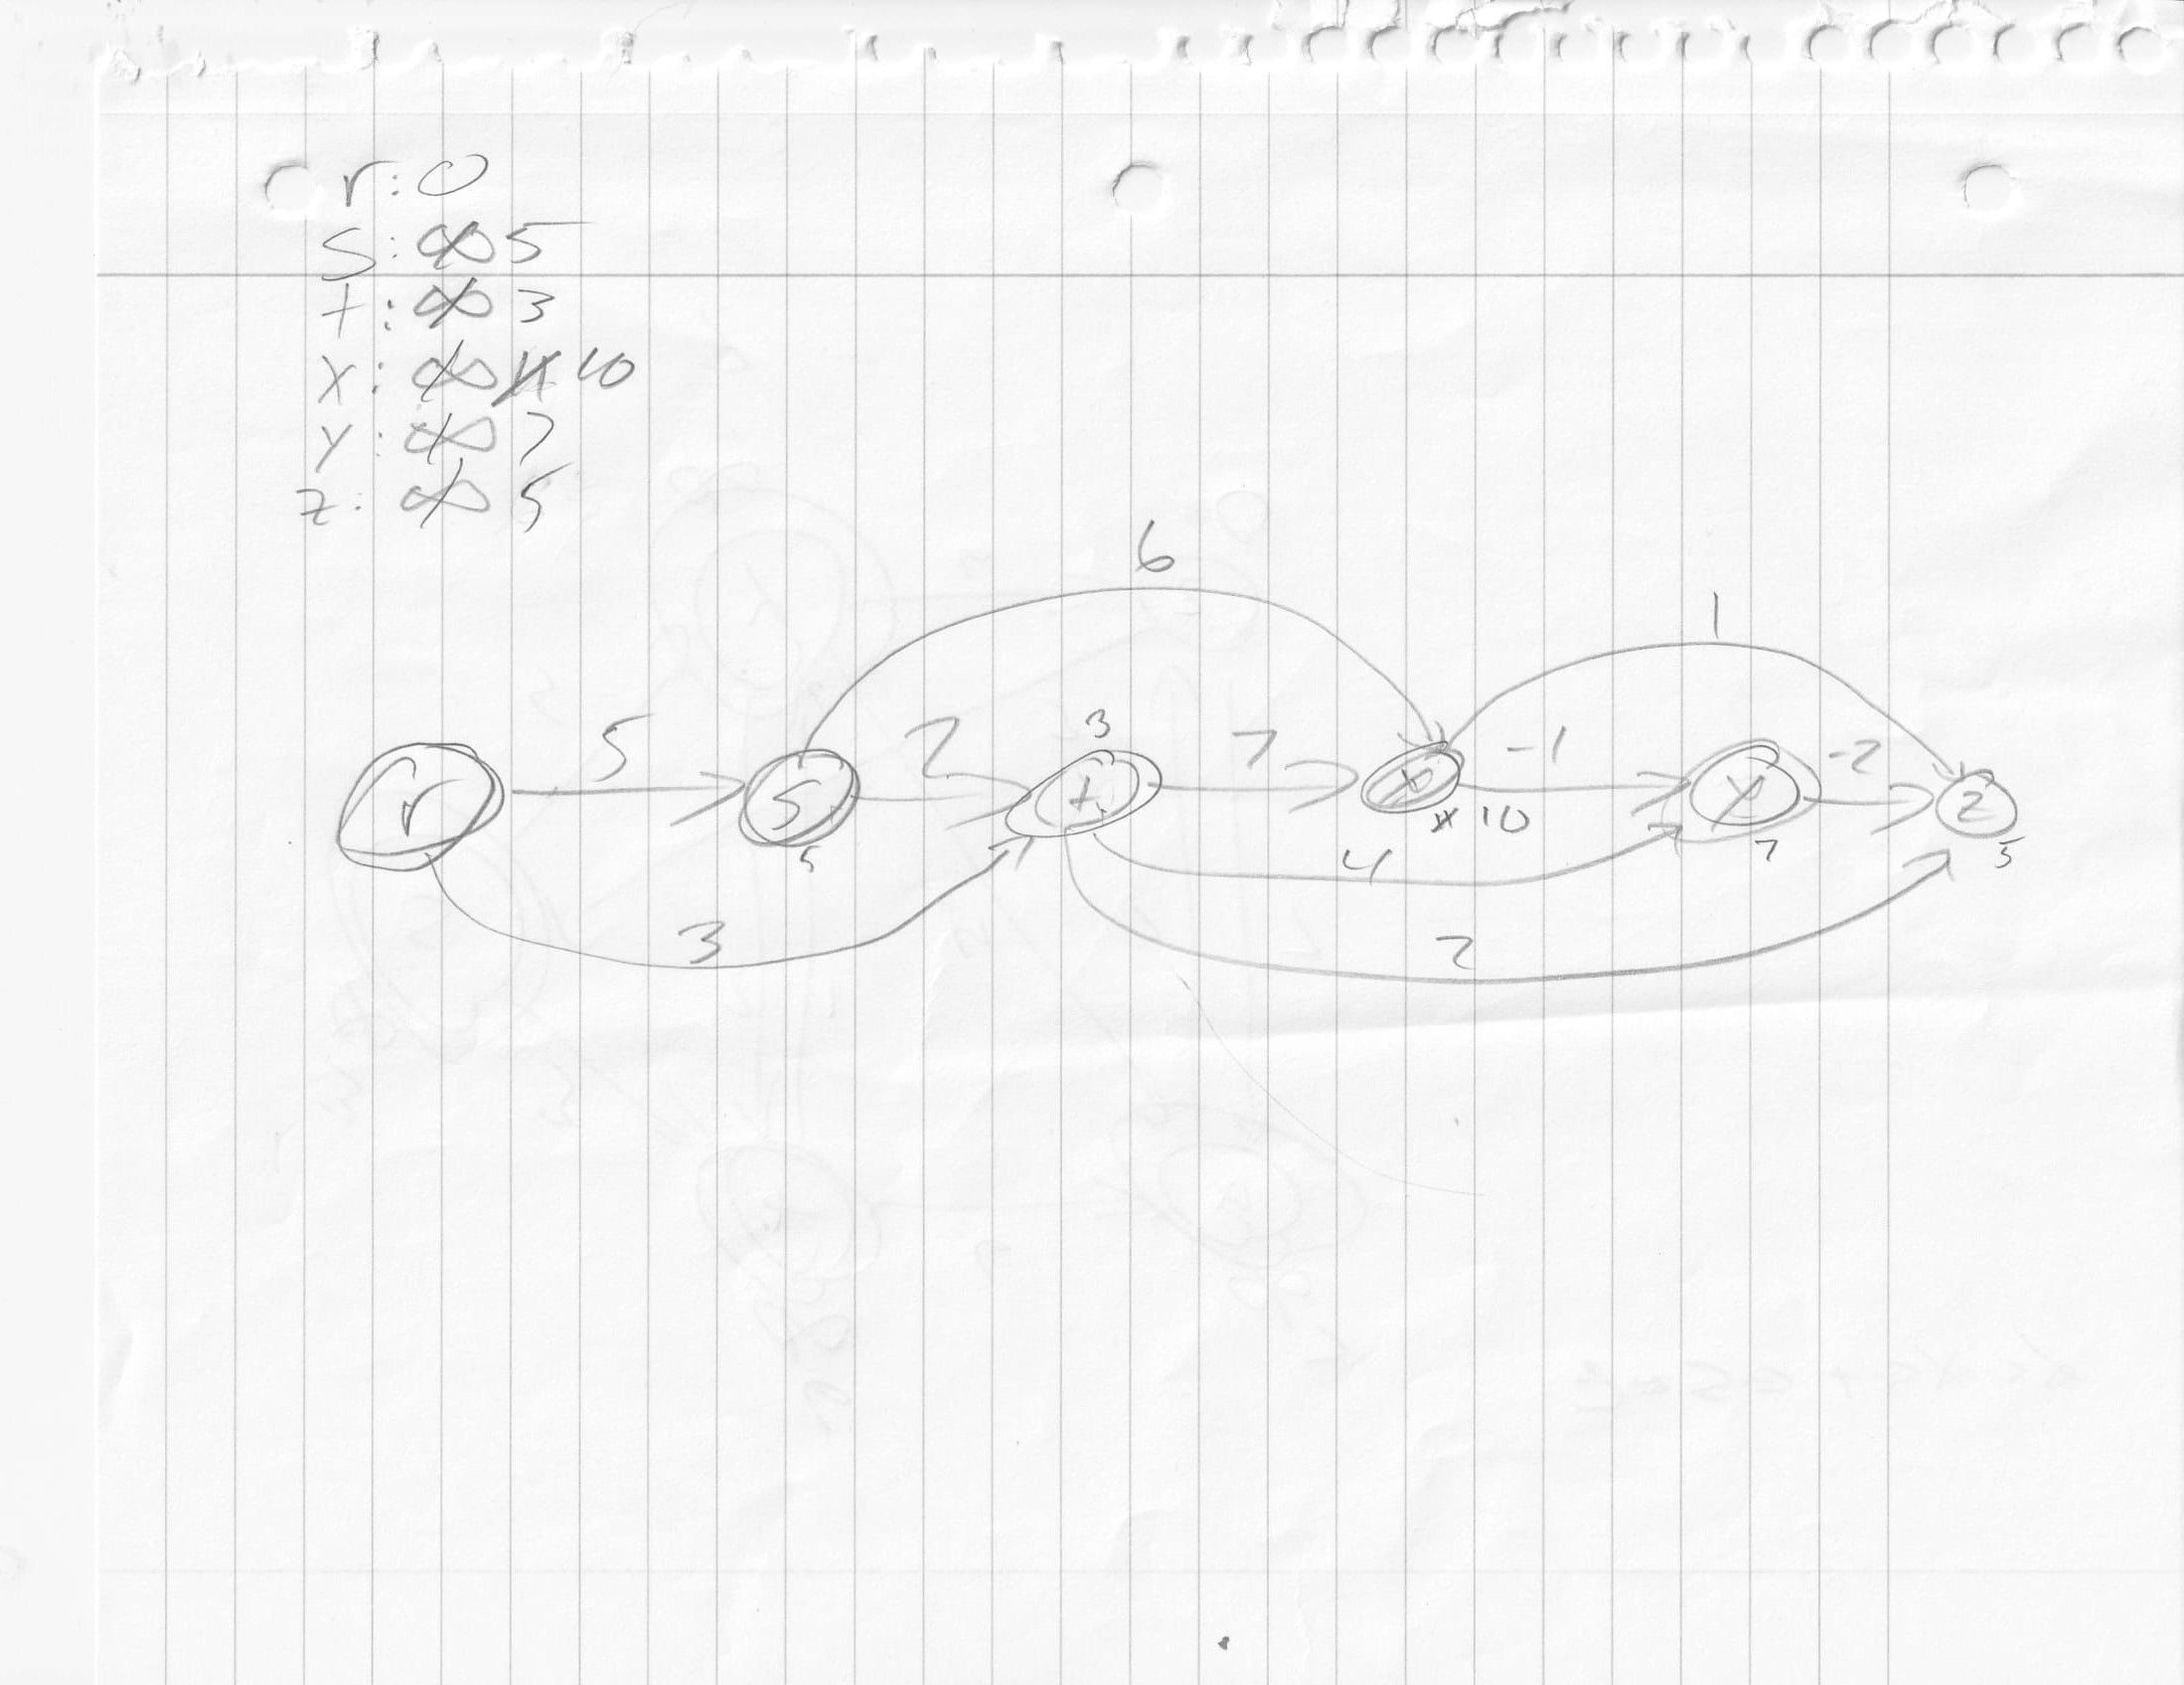
\includegraphics[scale=.32]{24.3-1.jpg}

\item Exercise 24.3-1 \\
Run Dijkstra’s algorithm on the directed graph of Figure 24.2, first using vertex s as the source and then using vertex z as the source. In the style of Figure 24.6, show the d and $\pi$ values and the vertices in set S after each iteration of the while loop.

Vertex s as source:
S is the source. T.d is 3 and y.d is 5, the set S is now $\{s\}$. T is selected as the next vertex since it's the shortest path. x.d is 9, S = $\{s,t\}$. Y is selected. z.d is 11, S = $\{s,t,y\}$. X is selected, S = $\{s,t,y,x\}$. Then z is selected, set S = $\{s,t,y,x,z\}$.\\
\begin{center}
 \begin{tabular}{|c|c c c c c|} 
 \hline
 Selected Vertex & s(d,$\pi$) & t(d,$\pi$) & x(d,$\pi$) & y(d,$\pi$) & z(d,$\pi$)\\ [0.5ex] 
 \hline
 NIL & 0,NIL &  $\infty$,NIL & $\infty$,NIL & $\infty$,NIL & $\infty$,NIL\\ 
 \hline
 s & 0,NIL & 3,NIL & $\infty$,NIL & 5,NIL & $\infty$,NIL\\ 
 \hline
 t & 0,NIL & 3,s & 9,NIL & 5,NIL & $\infty$,NIL \\
 \hline
 y & 0,NIL & 3,s & 9,NIL & 5,t & 11,NIL \\
 \hline
 x & 0,NIL & 3,s & 9,y & 5,t & 11,NIL \\
 \hline
 z & 0,NIL & 3,s & 9,y & 5,t & 11,x \\
 \hline
\end{tabular}
\end{center}
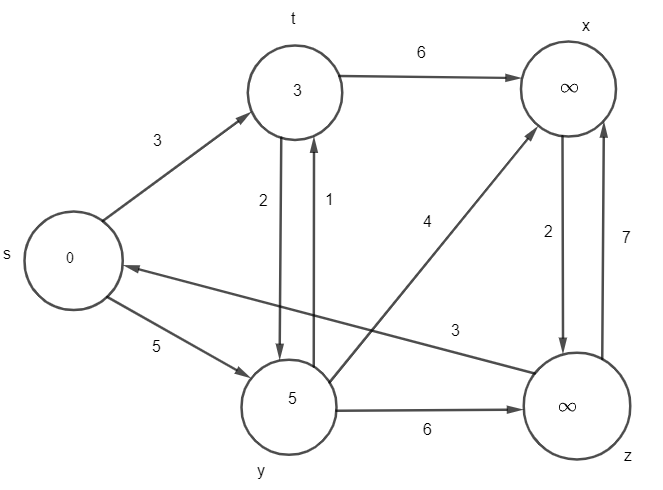
\includegraphics[scale=.65]{24.3-1 Vertex S/1-1.png}\\
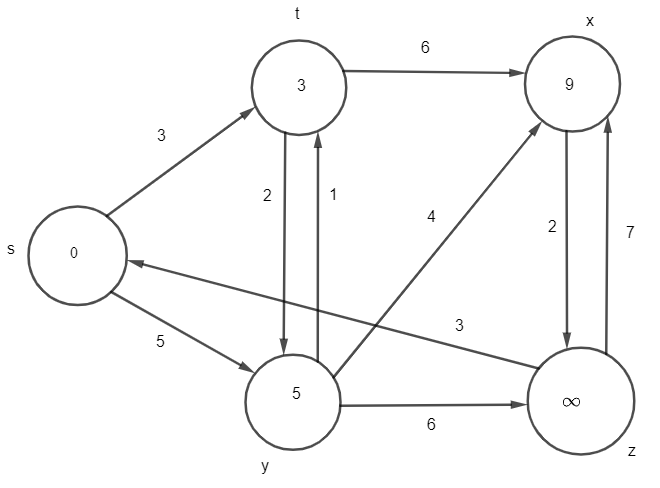
\includegraphics[scale=.65]{24.3-1 Vertex S/1-2.png}\\
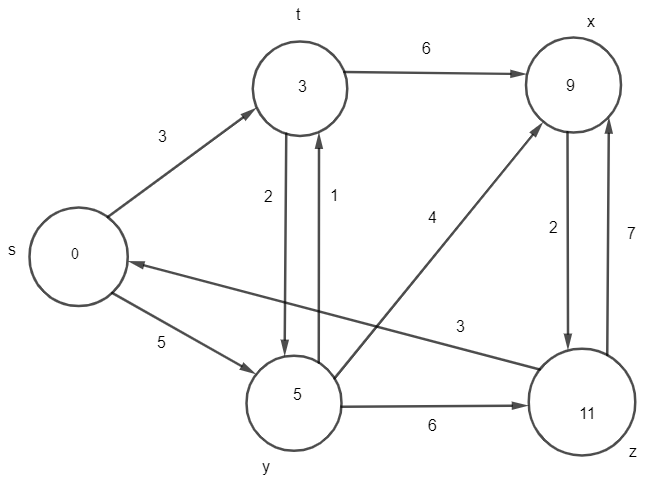
\includegraphics[scale=.65]{24.3-1 Vertex S/1-3.png}\\
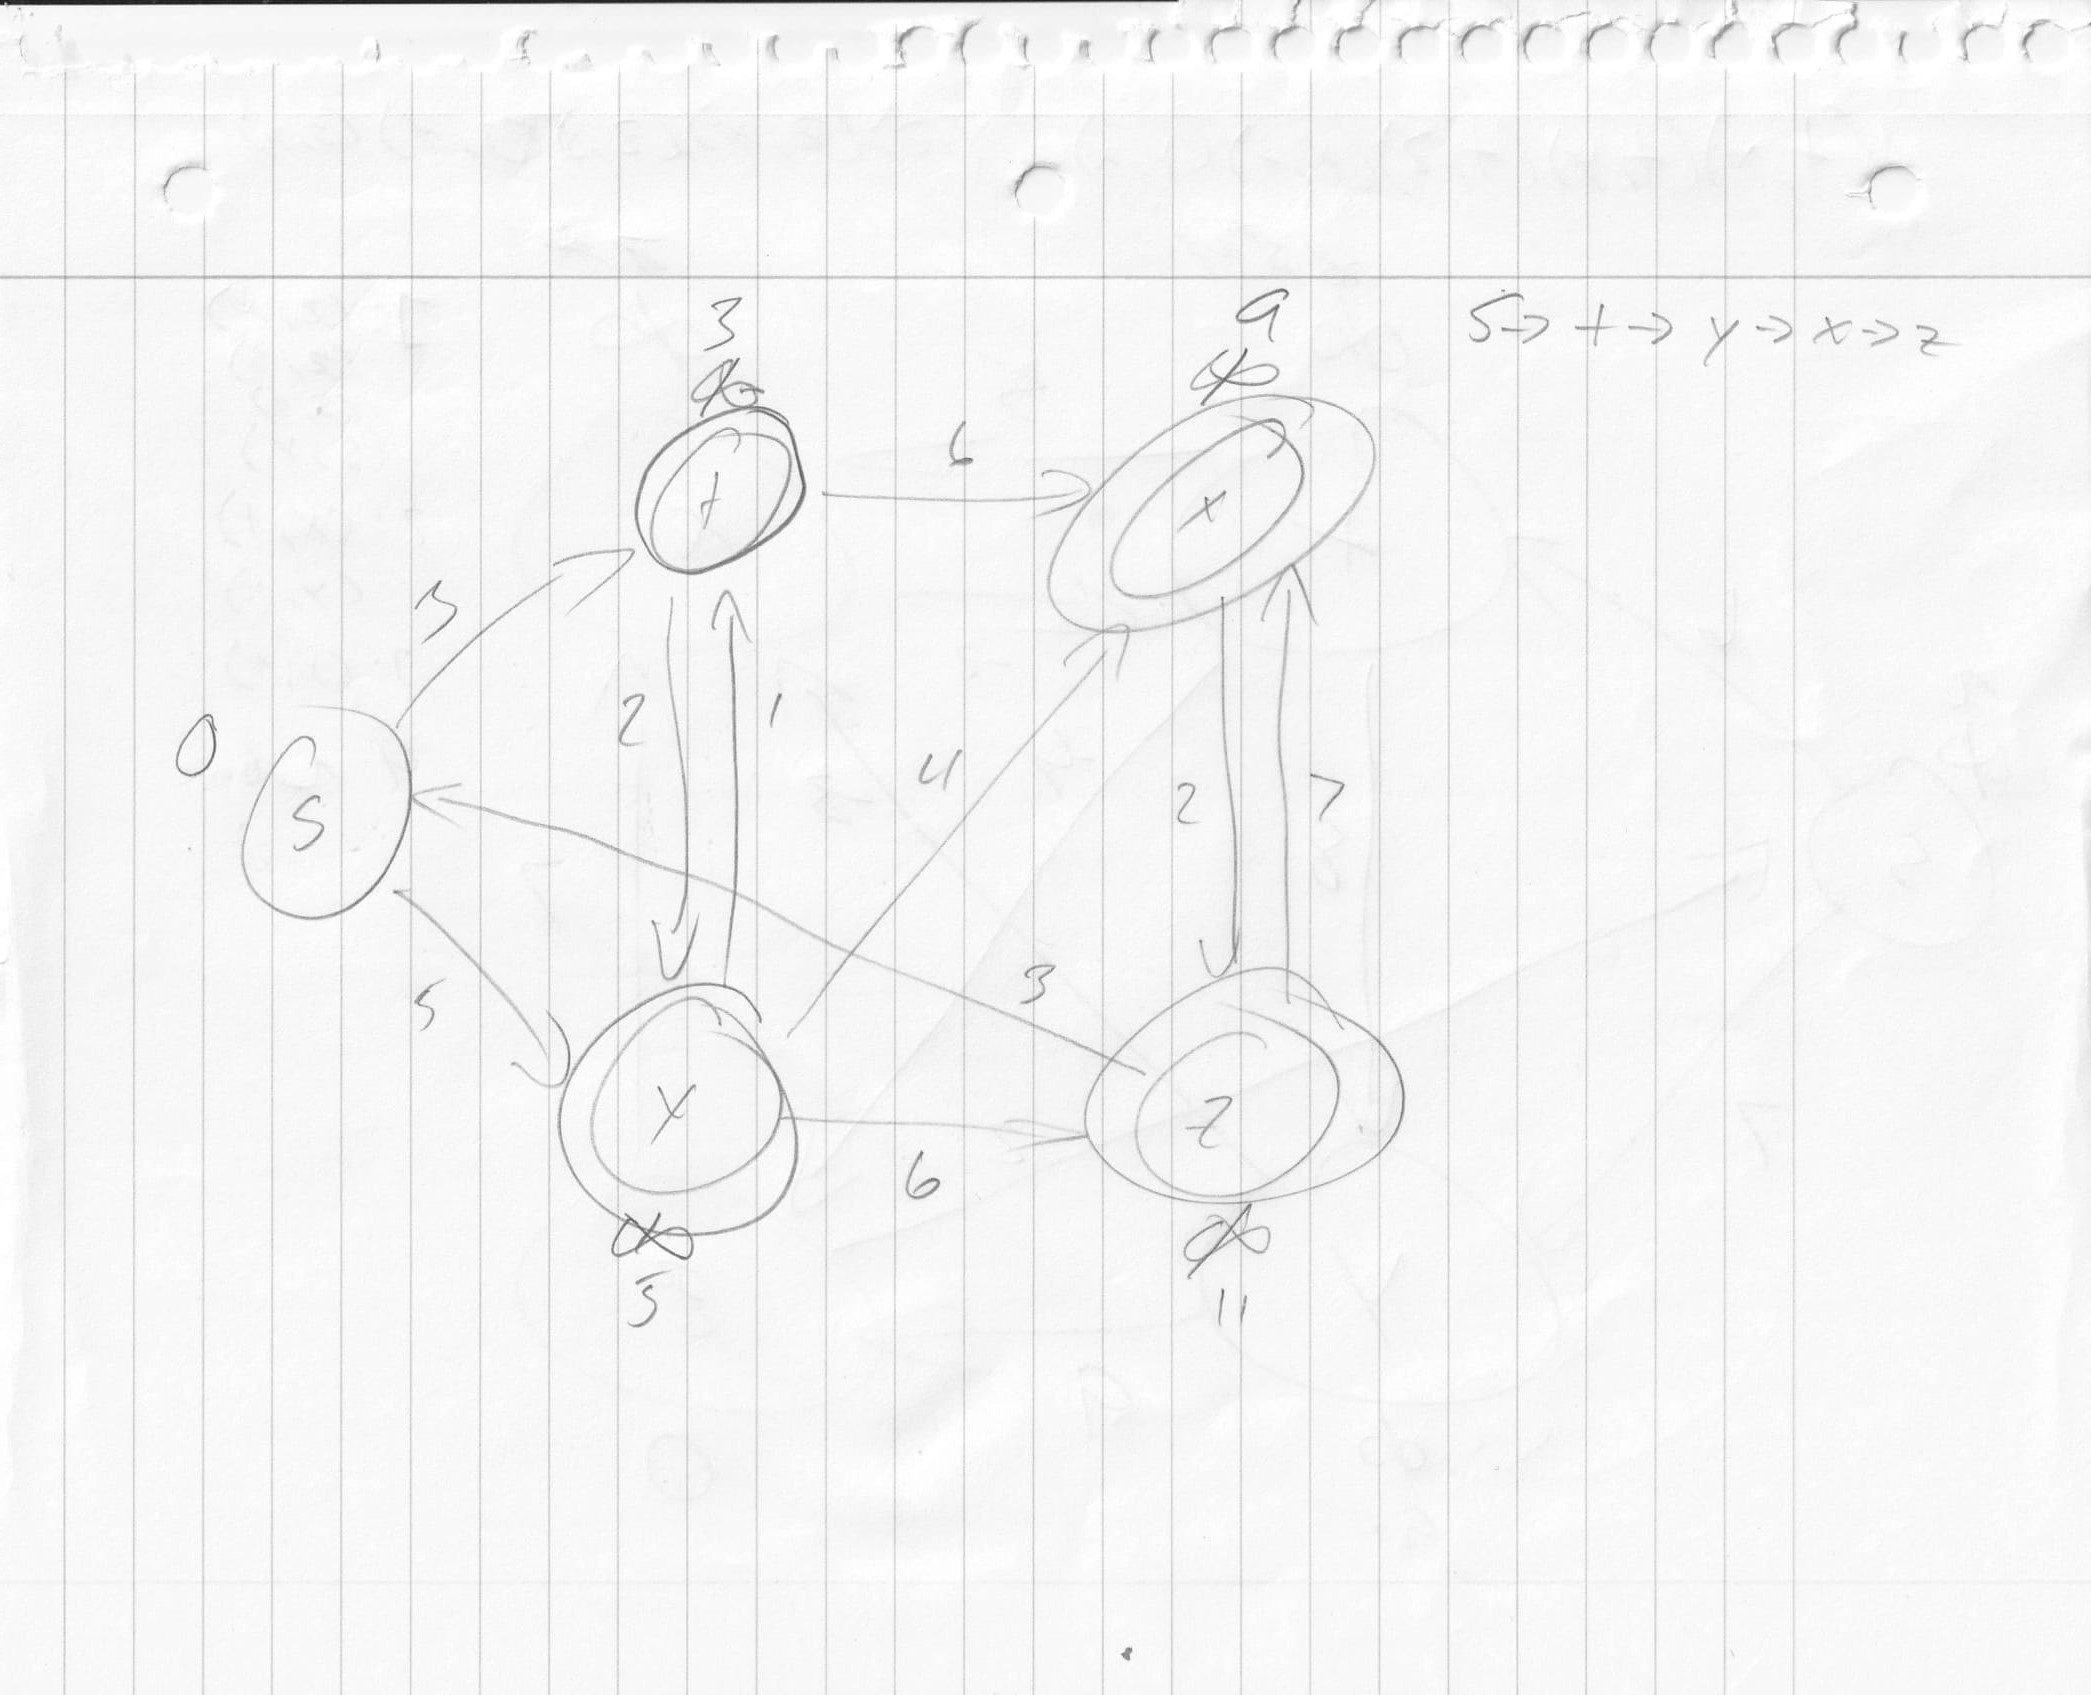
\includegraphics[scale=.32]{24.3-1 Vertex S/24.3-1S.jpg}\\

Vertex z as source:\\
Vertex Z is the source. s.d = 3  and x.d = 7, set S = $\{z\}$. Vertex S is selected. t.d = 6 and y.d = 8, S = $\{z,s\}$. Vertex T is selected. S = $\{z,s,t\}$. Vertex x is selected, S = $\{z,s,t,x\}$. Vertex Y is selected, S = $\{z,s,t,x,y\}$.
\begin{center}
 \begin{tabular}{|c|c c c c c|} 
 \hline
 Selected Vertex & s(d,$\pi$) & t(d,$\pi$) & x(d,$\pi$) & y(d,$\pi$) & z(d,$\pi$)\\ [0.5ex] 
 \hline
 NIL & $\infty$,NIL & $\infty$,NIL & $\infty$,NIL & $\infty$,NIL & 0,NIL\\ 
 \hline
 z & 3,NIL & $\infty$,NIL & 7,NIL & $\infty$,NIL & 0,NIL\\ 
 \hline
 s & 3,z & 6,NIL & 7,NIL & 8,NIL & 0,NIL \\
 \hline
 t & 3,z & 6,s & 7,NIL & 8,NIL & 0,NIL \\
 \hline
 x & 3,z & 6,s & 7,t & 8,NIL & 0,NIL \\
 \hline
 y & 3,z & 6,s & 7,t & 8,x & 0,NIL \\
 \hline
\end{tabular}
\end{center}
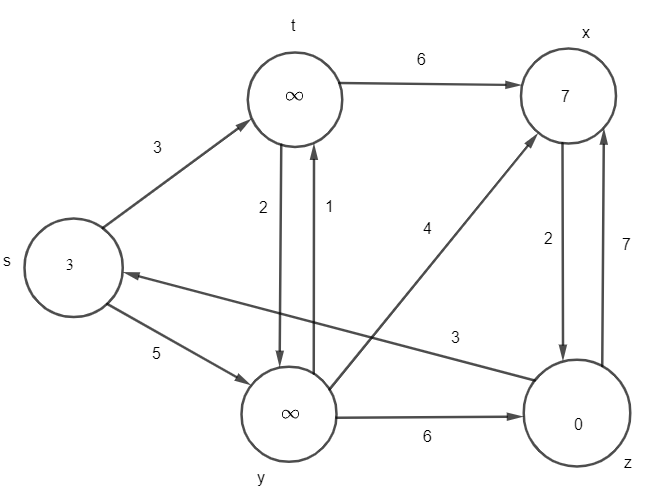
\includegraphics[scale=.65]{24.3-1 Vertex Z/2-1.png}\\
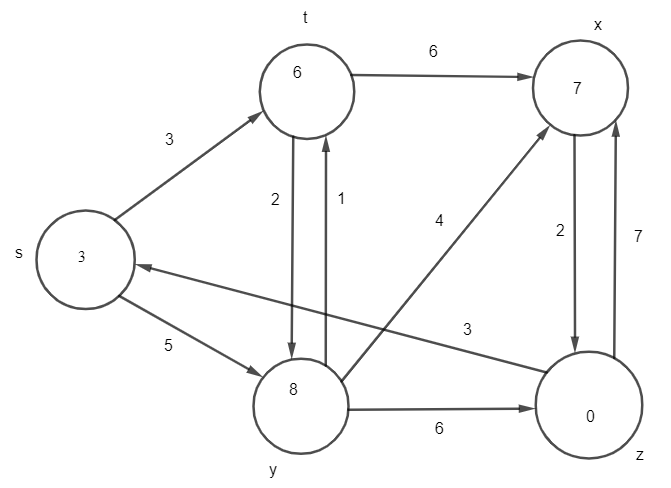
\includegraphics[scale=.65]{24.3-1 Vertex Z/2-2.png}\\
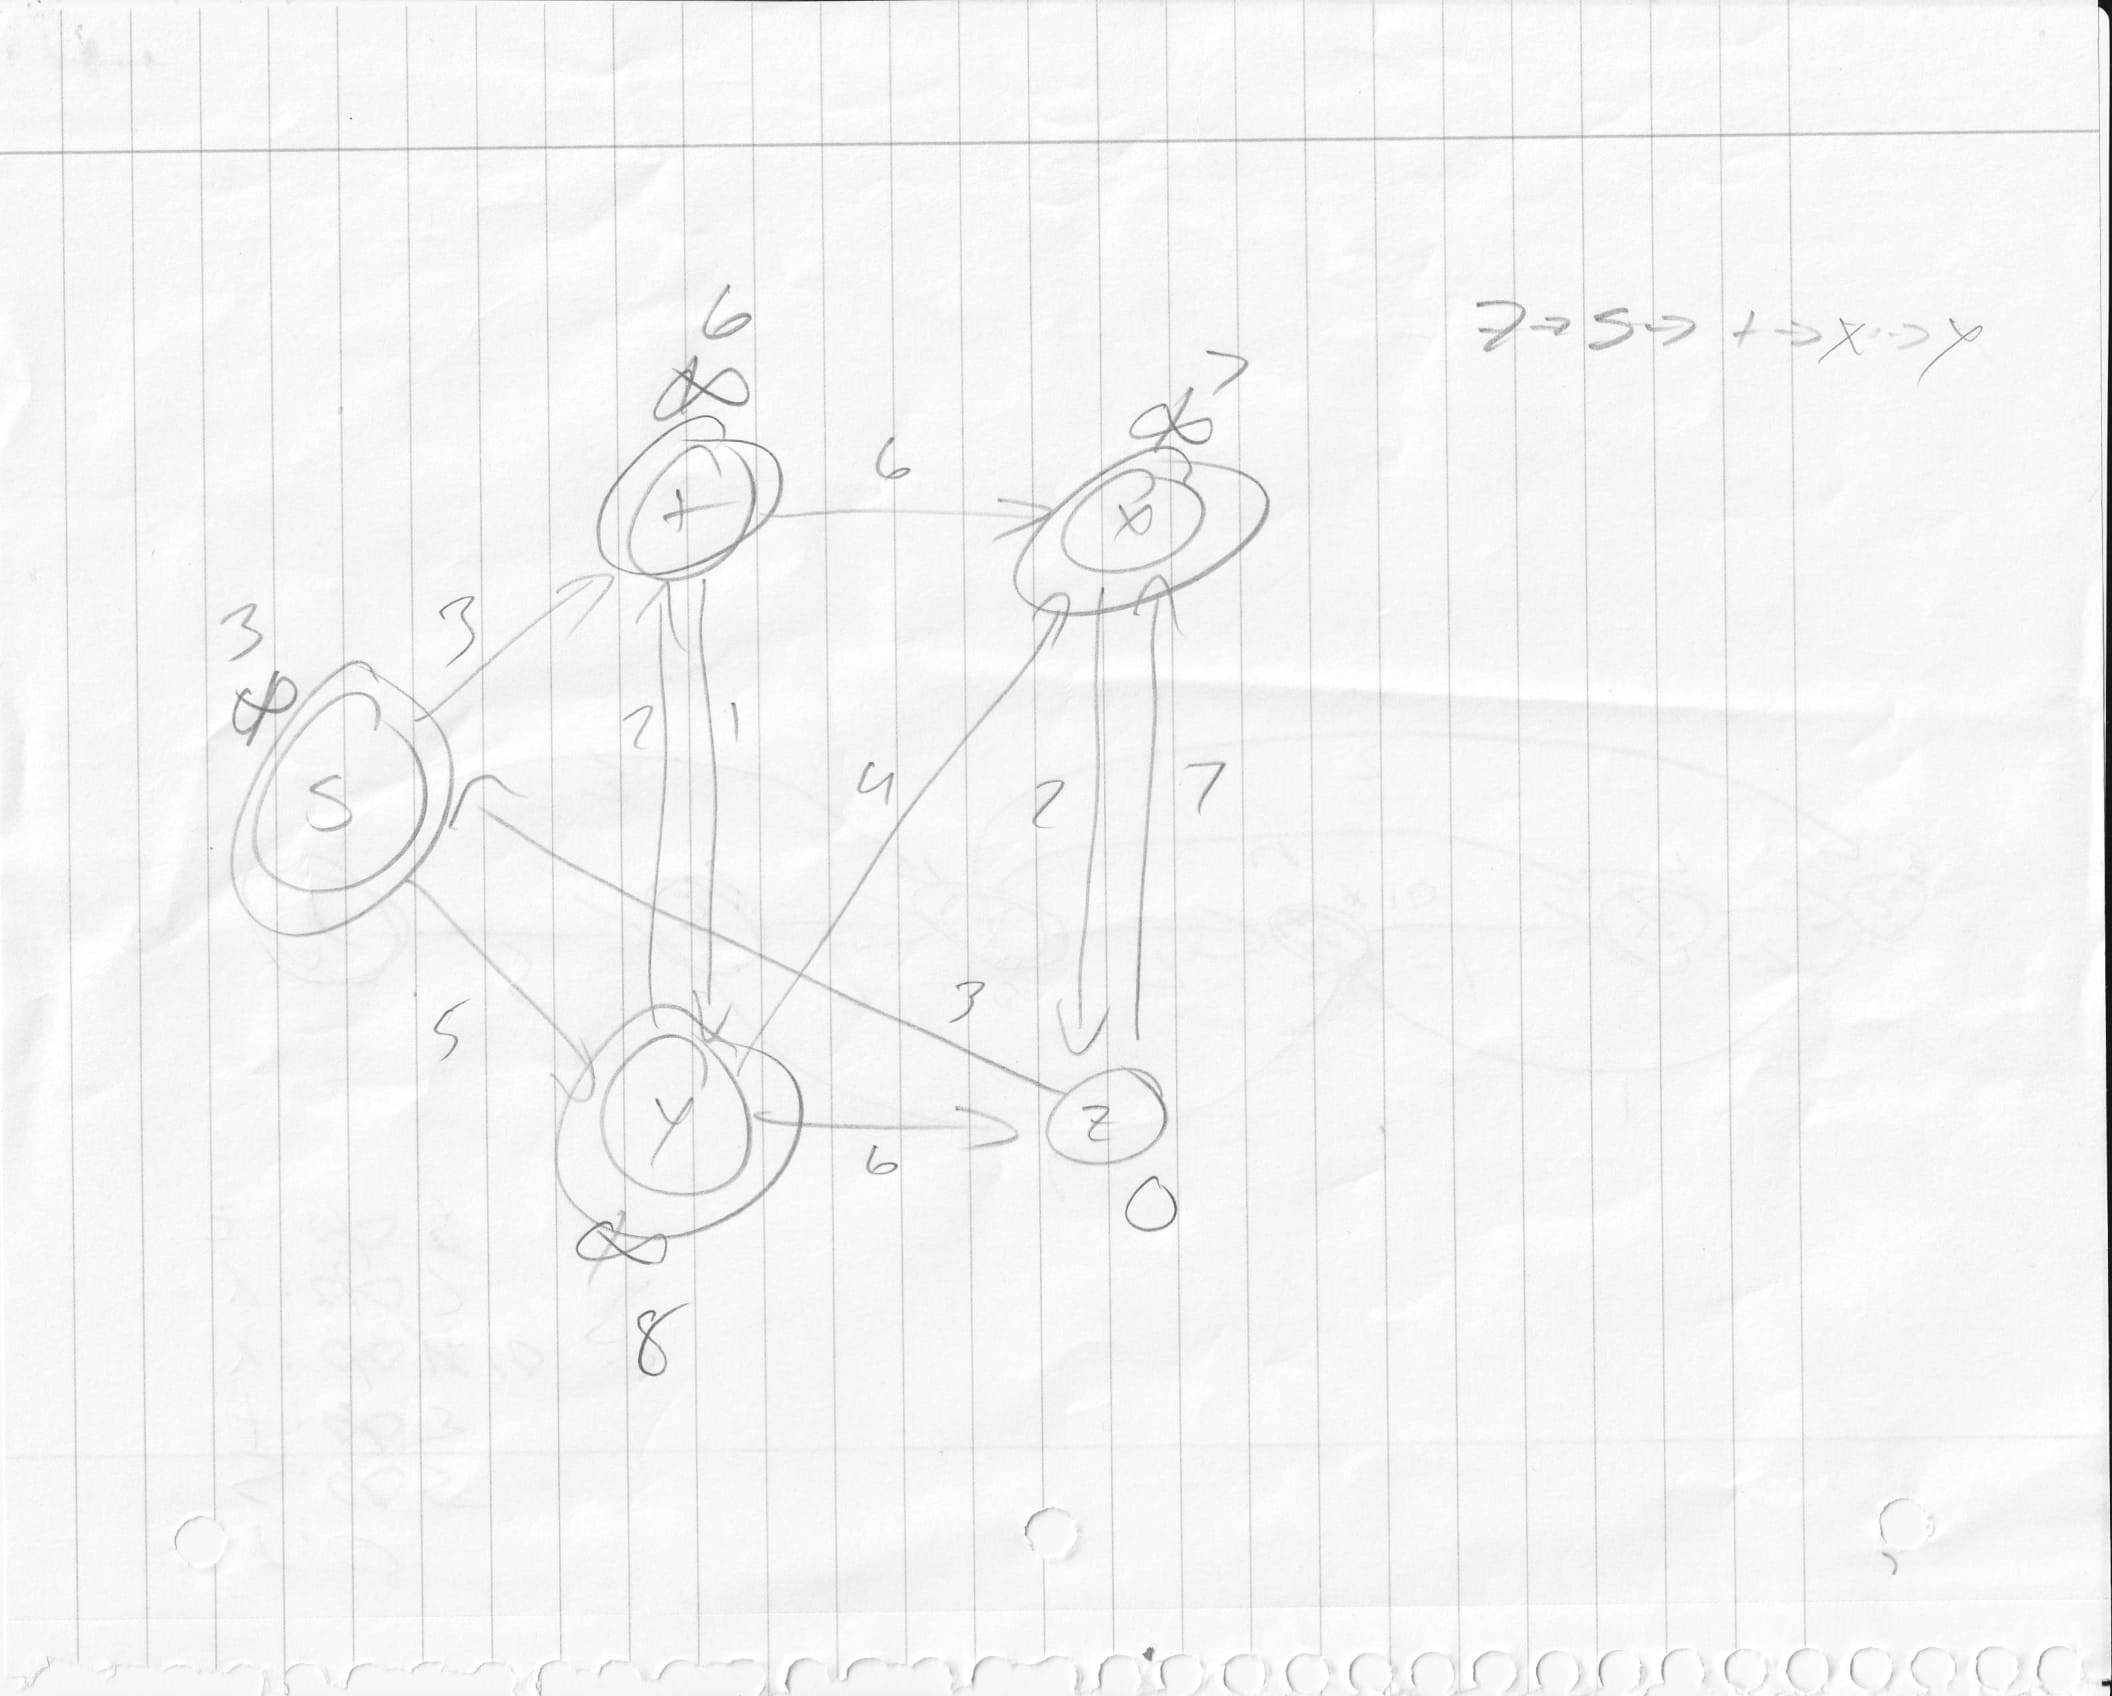
\includegraphics[scale=.32]{24.3-1 Vertex Z/24.3-Z.jpg}\\
\end{enumerate}
 
 
 Please email me if you have any questions.

% --------------------------------------------------------------
%     You don't have to mess with anything below this line.
% --------------------------------------------------------------
 
\end{document}